\section{Profilowanie oprogramowania - raport}

W celu przebadania opracowanego oprogramowania i skompilowanego programu pod względem wykonywania jego poszczególnych sekcji i występowania tzw. hot-spotów, wykorzystano narzędzie profilera dostępne w środowisku Visual Studio. \newline
Profiler pokazał, że najwięcej czasu procesor (program) spędza na wykonywaniu kroków algorytmu RK4 - sprawdzono czy zmienne służące do iterowania zadeklarowane jednorazowo jako pola klasy zamiast być tworzone z każdym obiegiem pętli skrócą w jakiś sposób czas wykonania programu. Wynik eksperymentu okazał się niejednoznaczy, jednak z całą pewnością można stwierdzić, że nie wpływa to na zużycie procesora.\newline
Poniżej na rysunku \ref{profiler1} przedstawiono wynik przeprowadzonego badania profilerem w środowisku Visual Studio.

\begin{figure}[ht!]
\centering
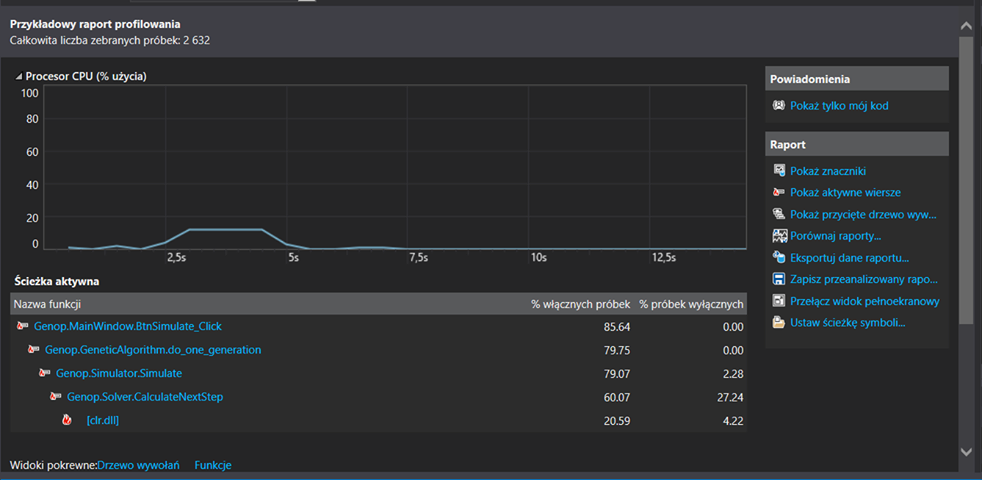
\includegraphics[scale=0.42]{profiler1}
\caption{Wynik przeprowadzonego testu występowania sekcji hot-spot}
\label{profiler1}
\end{figure} 

Optymalizacja funkcji \textit{CalculateNextStep} była niemożliwa z racji zachowania odpowiednich wymagań związanych z realizacją numerycznego rozwiązywania równań różniczkowych.\newline
Jednakże w metodzie \textit{simulate} wywyłującej symulację, znajdował się względnie nieefektywny algorytm obliczania błędu sygnału sterującego. Algorytm ten został zastąpiony wydajniejszą metodą - wyznaczaniem wartości całki uchybu sterowania, co spowodowało znaczące skrócenie czasu wykonywania całej symulacji co zauważyć można na rysunku \ref{profiler1}. \newline Wynik badania programu profilerem z zaimplementowanym nieoptymalnym algorytmem, przedstawiono na poniższym rysunku \ref{algorytm}.
\newpage

\begin{figure}[!ht]
\centering
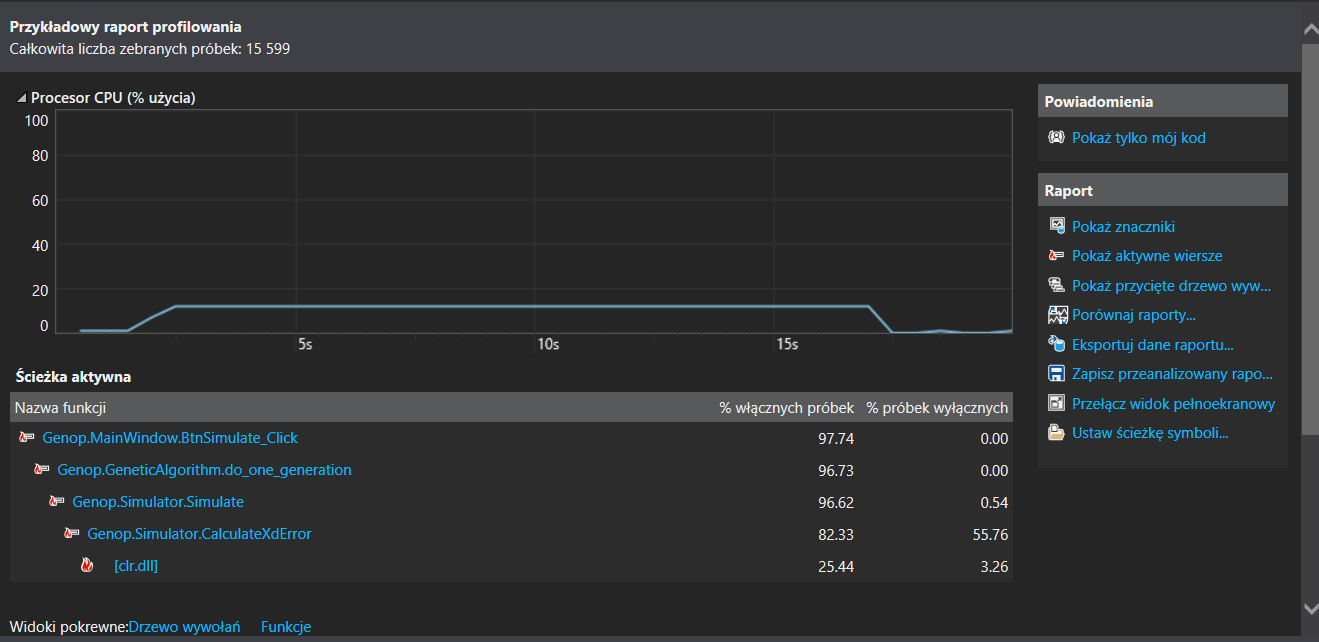
\includegraphics[scale=0.32]{algorytm}
\caption{Wynik badania profilerem z nieoptymalną sekcją programu}
\label{algorytm}
\end{figure} 
